\documentclass{experimentreport}

\input{listing_style.tex}

%========================
% 图表支持
%========================
\usepackage{graphicx}
\usepackage{float}
\usepackage{booktabs}
\usepackage{caption}
\usepackage{subcaption}
\captionsetup{font=small,labelfont=bf,labelsep=quad}
\graphicspath{{../results/figures/}}

%========================
% 基本信息
%========================

\setcoursename{基础软件开发技术实践}
\setreportname{智能软件工程实验报告}

\setexperimenttitle{实验一：代码审查意见挖掘与需求理解}

\setstudentname{\hintholder{王皓}}
\setdepartment{\hintholder{计算学部}}
\setstudentid{\hintholder{2023111825}}

\setcourseteacher{刘佳琨}
\setinstructor{刘佳琨}

\setlablocation{\hintholder{格物213}}
\setlabtime{    \hintholder{2026年6月29日}}

\begin{document}

%========================
% 自动生成封面
%========================

\makereporthead

%========================
% 实验目的
%========================

\experimentpurpose{

完成本实验后，学生应能够：

\begin{enumerate}
  \item 理解现代软件开发过程中 Pull Request（PR）与 Code Review 的基本流程。
  \item 熟悉 GitHub 开源软件仓库中代码审查数据的组织形式。
  \item 掌握 Pull Request、Commit、Review、Comment 等对象之间的关系。
  \item 能够利用 GitHub API 或公开数据集获取代码审查数据。
  \item 能够完成代码、文本及元数据等多源信息的抽取。
  \item 掌握数据集统计分析方法，为后续模型训练提供数据基础。
\end{enumerate}

}

%========================
% 实验内容
%========================

\experimentcontent{

本实验的工作可概括为一条完整的数据流水线：\textbf{目标选择 $\rightarrow$ 数据采集 $\rightarrow$ 特征与标签抽取 $\rightarrow$ 清洗与建模 $\rightarrow$ 探索性分析}。下面依次说明各环节的设计与实现。

\subsection*{2.1 目标仓库选择}

代码审查数据的质量首先取决于数据来源。为使采集到的数据能够同时支撑后续七个实验，本实验依据四条准则筛选目标仓库：（1）\textbf{以 Python 为主语言}，使实验二的 AST/CFG 解析与实验三的 Code2Vec/CodeBERT 表示学习可以统一处理，避免为多种语言分别实现解析器；（2）\textbf{PR 量大、审查文化成熟}，以保证带 \texttt{diff\_hunk} 的 inline 审查评论足够多，为实验三的生成任务提供训练配对；（3）\textbf{存在 bot/AI 活动痕迹}，使实验五能筛出足量 AI 生成代码与 AI 审查者样本；（4）\textbf{覆盖不同开源社区}，以呼应实验一的拓展目标——分析不同社区代码审查流程的差异。

据此最终选定 5 个大型仓库，覆盖 Web 框架、数据科学、机器学习、基础设施与物联网五个领域：\texttt{django/\allowbreak django}、\texttt{pandas-dev/\allowbreak pandas}、\texttt{huggingface/\allowbreak transformers}、\texttt{apache/\allowbreak airflow} 与 \texttt{home-assistant/\allowbreak core}。

\subsection*{2.2 数据采集}

采集环节仅抓取\textbf{已关闭}（closed）的 PR，即包含已合并（merged）与关闭未合并（closed-unmerged）两类，而不采集开放中的 PR。这一决策直接服务于合并预测任务：开放 PR 的最终结局未知，纳入会污染标签；已关闭 PR 结局已定，合并为正例、关闭未合并为负例，标签天然干净。

对每个 PR，通过 GitHub REST API 抓取六类子资源并打包为独立 JSON 文件：PR 详情（\texttt{detail}）、改动文件与 diff（\texttt{files}）、正式审查（\texttt{reviews}）、inline 审查评论（\texttt{review\_comments}）、对话区评论（\texttt{issue\_comments}）与提交记录（\texttt{commits}）。为应对 GitHub 的限流约束（认证后核心 API 限额 5000 次/小时），客户端实现了三项机制：额度耗尽时读取 \texttt{X-RateLimit-Reset} 头精确休眠至额度恢复、二级限流与 5xx 错误时指数退避重试、以及基于 \texttt{Link} 头的自动翻页。由于每个 PR 独立存盘且抓取前先检查文件是否存在，整个采集过程支持\textbf{断点续传}，可随时中断续跑而不重复消耗额度。

考虑到 AI 生成代码的 PR 在自然分布中极为稀少（约 2\%–5\%），若仅靠随机抽样将导致实验五样本不足，因此在每仓库 300 条基础样本之外，额外使用 Search API 定向补采带 AI 信号的 PR（每仓库上限 50 条），并以 \texttt{oversampled} 字段标记，以便后续分析时区分自然分布与人为补采。

\subsection*{2.3 特征与标签抽取}

在原始数据之上抽取三类信息。\textbf{统计特征}包括代码改动量（additions/deletions/changed\_files）、提交数、审查次数、审查者人数、inline 评论数、对话评论数与标签数，可供实验二直接使用。\textbf{预测标签}以 \texttt{is\_merged} 为核心因变量，并保留 \texttt{review\_decision}（APPROVED、CHANGES\_REQUESTED、COMMENTED、NONE 四类）。\textbf{AI 标签}拆分为两个相互独立的启发式标签：\texttt{is\_ai\_code} 判定代码是否由 AI 辅助生成，\texttt{has\_ai\_reviewer} 判定是否有 AI 参与审查。二者均采用分强弱的多信号判定——强信号如 commit 或 PR 正文中的 \texttt{Co-authored-by} 署名（署名对象为已知 AI 工具）、代码生成 bot 作者、已知 AI 审查 bot 账号；弱信号如 AI 相关标签、正文文本提及——并将命中的具体信号写入 \texttt{ai\_code\_signals} 与 \texttt{ai\_reviewer\_signals} 字段，以便人工复核与高精度子集筛选。

\subsection*{2.4 数据清洗与关系型建模}

考虑到不同实验需要不同粒度的数据，若组织为单一扁平宽表既浪费存储又难以使用，因此本数据集采用\textbf{关系型多表结构}，由 5 张表通过 \texttt{repo + number} 联结：主表 \texttt{prs}（每 PR 一行）、\texttt{files}（每改动文件一行）、\texttt{reviews}（每条正式审查一行）、\texttt{review\_comments}（每条 inline 评论一行）与 \texttt{commits}（每个提交一行）。清洗规则包括：丢弃无文件改动的 PR、按 \texttt{repo+number} 去重、对过大而无 diff 的文件保留文件行但置 \texttt{has\_patch=False}、按扩展名识别文件语言、逐 PR 调用启发式逻辑写入 AI 标签。每张表同时存为 \texttt{.parquet}（供后续实验高效读取）与 \texttt{.csv}（供人工查看）两份。

\subsection*{2.5 探索性数据分析}

最后对构建完成的数据集进行探索性分析，围绕指导书步骤五的要求，从合并结果、审查评论、标签、审查者、PR 规模、AI 参与与跨仓库差异等维度进行统计与可视化，识别数据分布特征及其对下游建模的影响。分析结果详见第三部分。

}

%========================
% 实验结果
%========================

\experimentresult{

按照上述流水线，最终构建的数据集共包含 \textbf{1{,}706 条}有效 PR，来自 5 个仓库；其余各表规模为 \texttt{files} 14{,}158 行、\texttt{review\_comments} 3{,}194 行、\texttt{commits} 4{,}549 行。表~\ref{tab:scale} 给出数据集的总体规模。本部分按"合并结果 $\rightarrow$ 审查活动 $\rightarrow$ PR 规模 $\rightarrow$ AI 参与 $\rightarrow$ 跨仓库差异"的顺序，结合可视化结果依次展开分析。每项分析均遵循"分析方法 $\rightarrow$ 观察到的现象 $\rightarrow$ 得出的结论"的逻辑链条。

\begin{table}[H]
\centering
\caption{数据集总体规模}
\label{tab:scale}
\small
\begin{tabular}{lrl}
\toprule
表 & 行数 & 说明 \\
\midrule
\texttt{prs}             & 1{,}706  & 有效 PR（基础 1{,}498 + 净补采 208） \\
\texttt{files}           & 14{,}158 & 平均每 PR 约 8.3 个改动文件 \\
\texttt{review\_comments} & 3{,}194  & inline 审查评论 \\
\texttt{commits}         & 4{,}549  & 平均每 PR 约 2.67 个提交 \\
\bottomrule
\end{tabular}
\end{table}

\subsection*{3.1 数据集综合概览}

在数据可视化阶段，为把握数据集全貌，首先绘制了综合概览图（图~\ref{fig:overview}），覆盖合并结果、审查评论、PR 规模、审查者、审查决策、作者身份、仓库分布、AI 参与与 PR 生命周期九个维度。该图显示，数据集在各维度上均具备充分的多样性：作者身份覆盖从核心成员（MEMBER）到外部贡献者（NONE）的完整谱系，审查决策以 APPROVED（962 条）为主、显式拒绝（CHANGES\_REQUESTED，80 条）较少，PR 生命周期中位数仅 9.5 小时但呈明显长尾（p90 $\approx$ 180 小时）。这一概览为后续分维度分析提供了整体背景。

\begin{figure}[H]
\centering
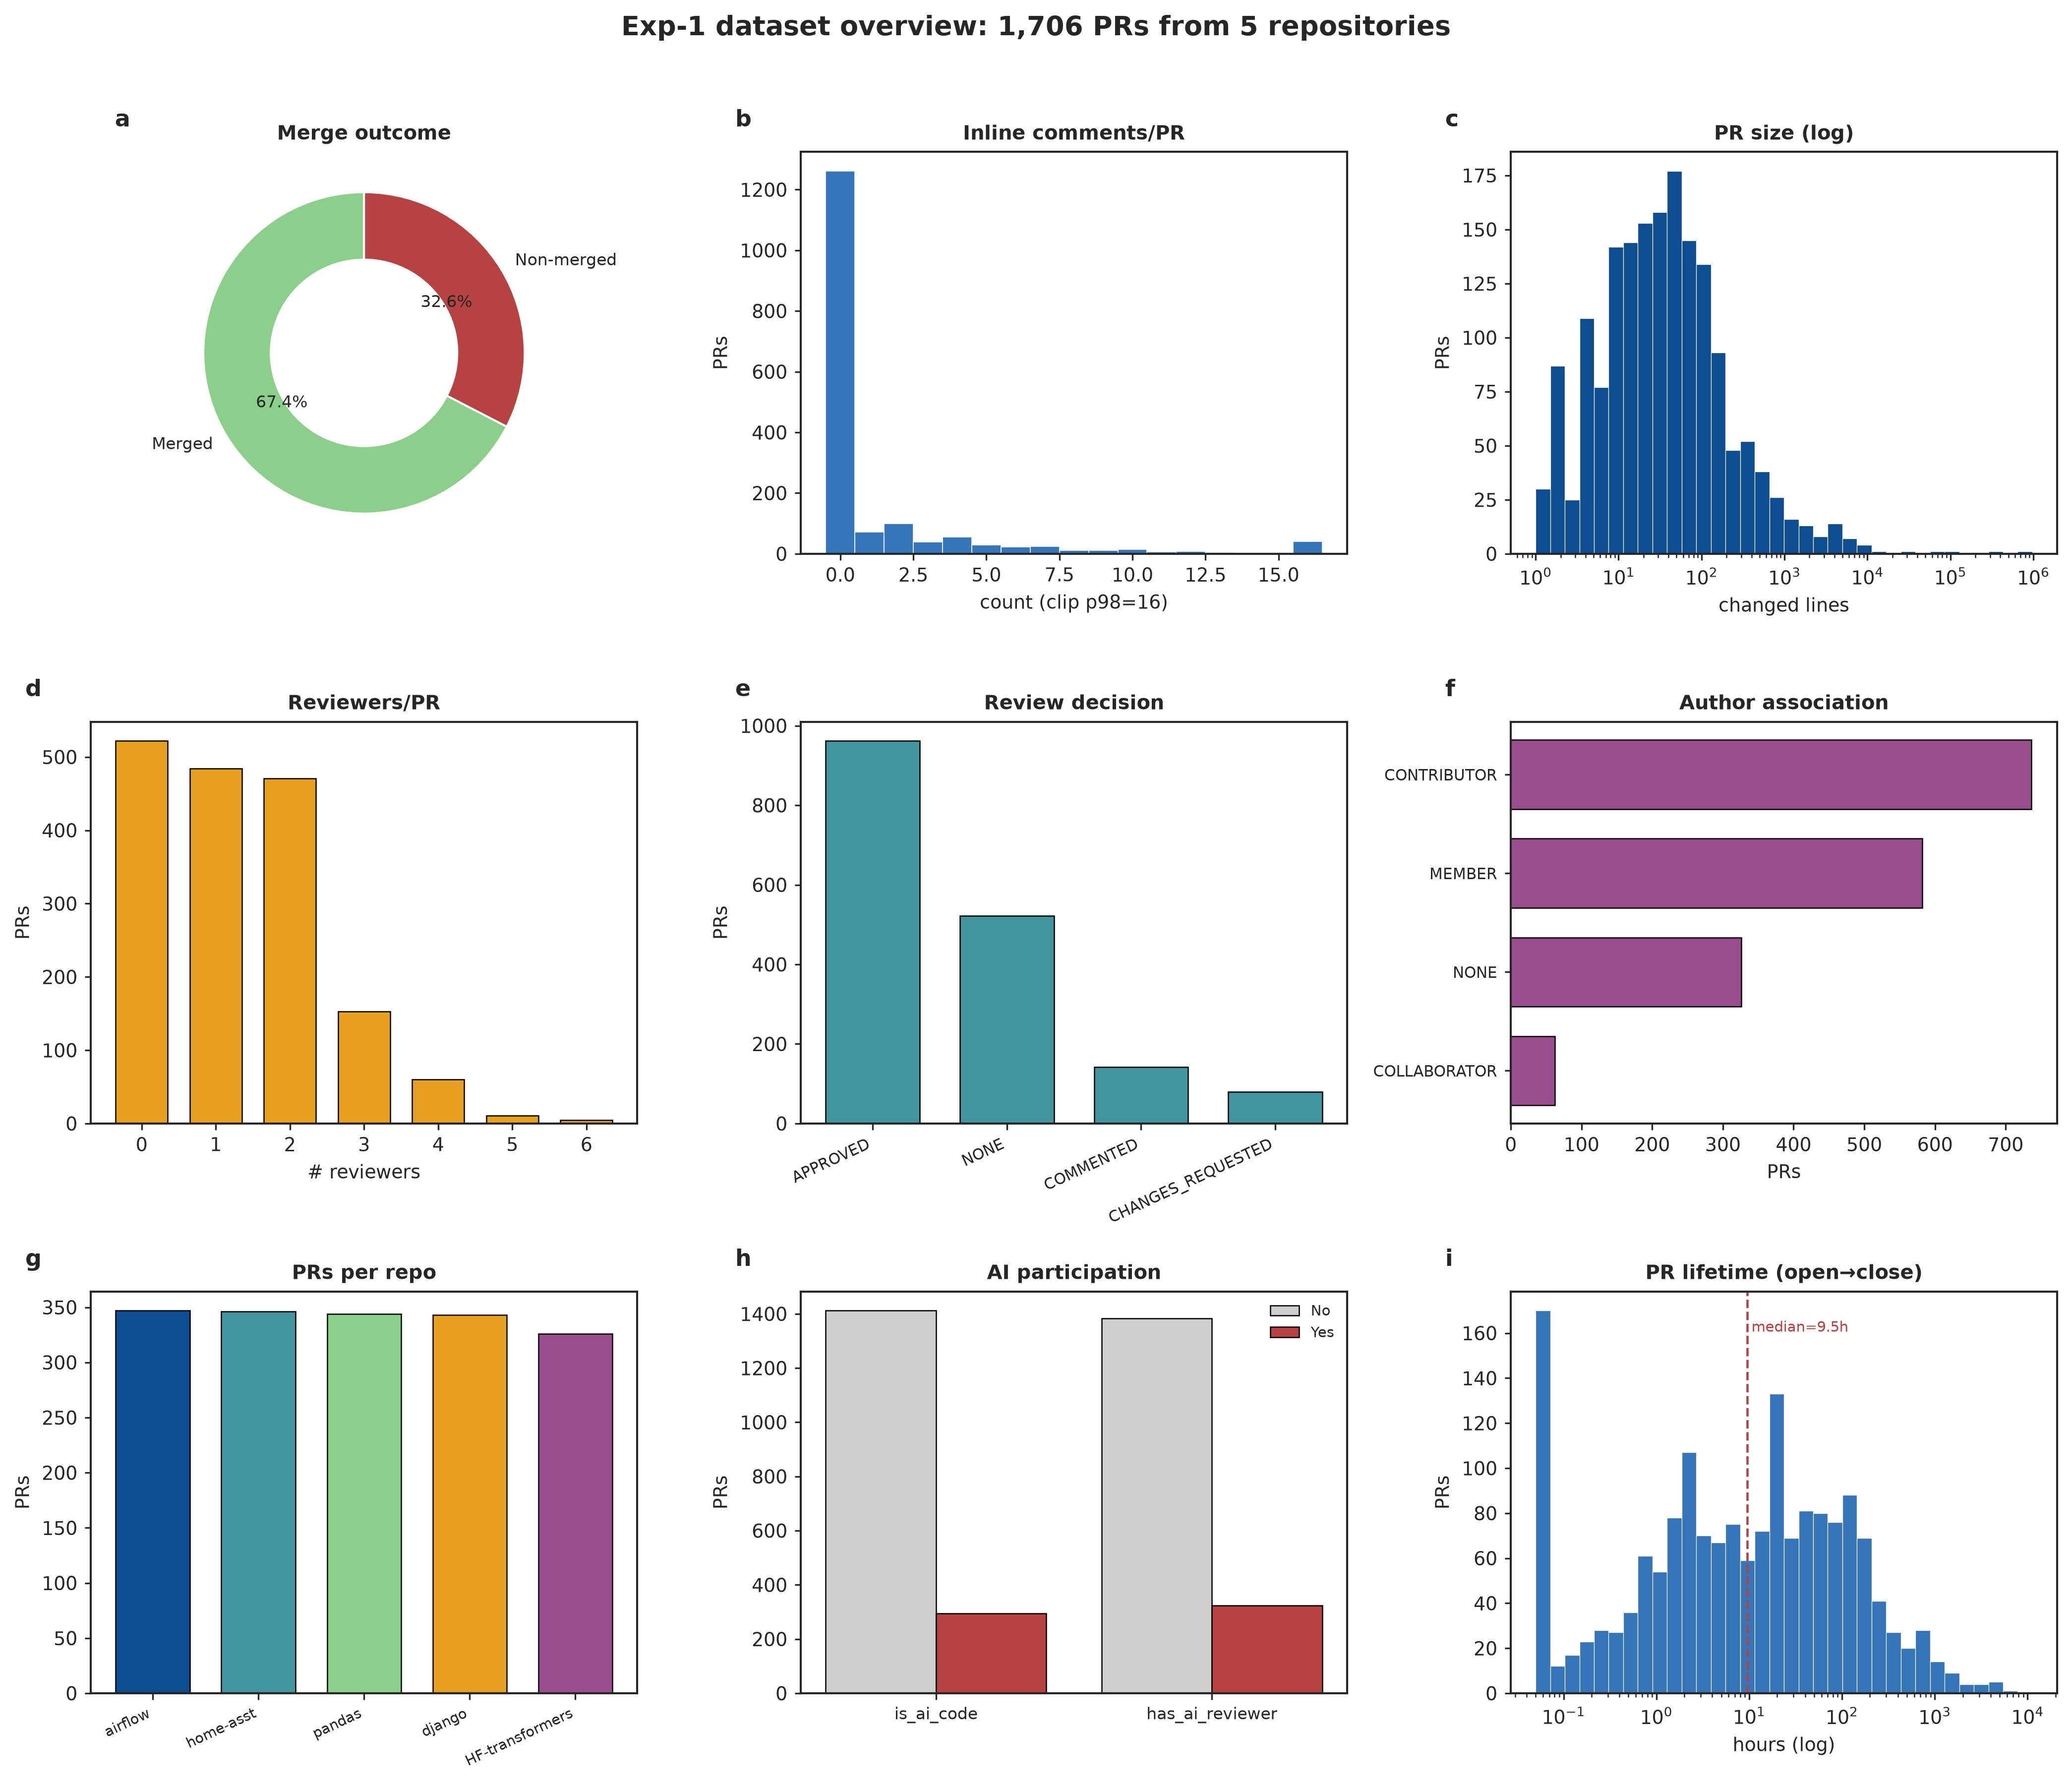
\includegraphics[width=0.92\textwidth]{eda_overview.png}
\caption{\textbf{实验一数据集综合概览。} 覆盖数据集九个关键维度（$N=1{,}706$ 条 PR，5 个仓库，2015--2026）：(a) 合并结果占比；(b) inline 评论数分布（截尾至 p98）；(c) PR 规模（对数）；(d) 审查者数量分布；(e) 正式审查决策；(f) 作者身份；(g) 各仓库 PR 数量；(h) AI 参与（\texttt{is\_ai\_code}/\texttt{has\_ai\_reviewer}）；(i) PR 生命周期（对数，中位数 9.5 小时）。多个维度共享长尾特征，提示后续建模需系统性地进行对数或分位数变换。}
\label{fig:overview}
\end{figure}

\subsection*{3.2 合并结果分布与类别不平衡}

合并状态 \texttt{is\_merged} 是合并预测任务的目标变量，其分布决定了分类问题的难度。统计合并与未合并 PR 的数量、比例，并进一步按仓库分组计算合并率（图~\ref{fig:merge}）。结果显示，全体 1{,}706 条 PR 中 1{,}150 条（67.4\%）被合并、556 条（32.6\%）未合并，正负样本比约 2:1，属于\textbf{轻度类别不平衡}。更关键的是，各仓库合并率差异极为显著：\texttt{home-assistant/core} 高达 90.2\%，而 \texttt{django/django} 仅 47.8\%，跨度超过 42 个百分点。这一现象反映了不同社区迥异的准入文化——django 以严格审查、反复修改著称，home-assistant 则更多依赖自动化测试与 bot 审查而快速合并。

由此得出两点对后续实验的结论：其一，整体 2:1 的不平衡要求实验二/三在划分数据集时采用分层采样，或在损失函数中引入类别权重；其二，仓库间超过 40 个百分点的合并率差异意味着存在显著的\textbf{分布偏移}，跨仓库训练/测试将严重影响模型泛化，故后续实验应按仓库分层划分或将仓库作为协变量处理。此即指导书思考题 5 所指的类别不平衡问题的具体表现与应对。

\begin{figure}[H]
\centering
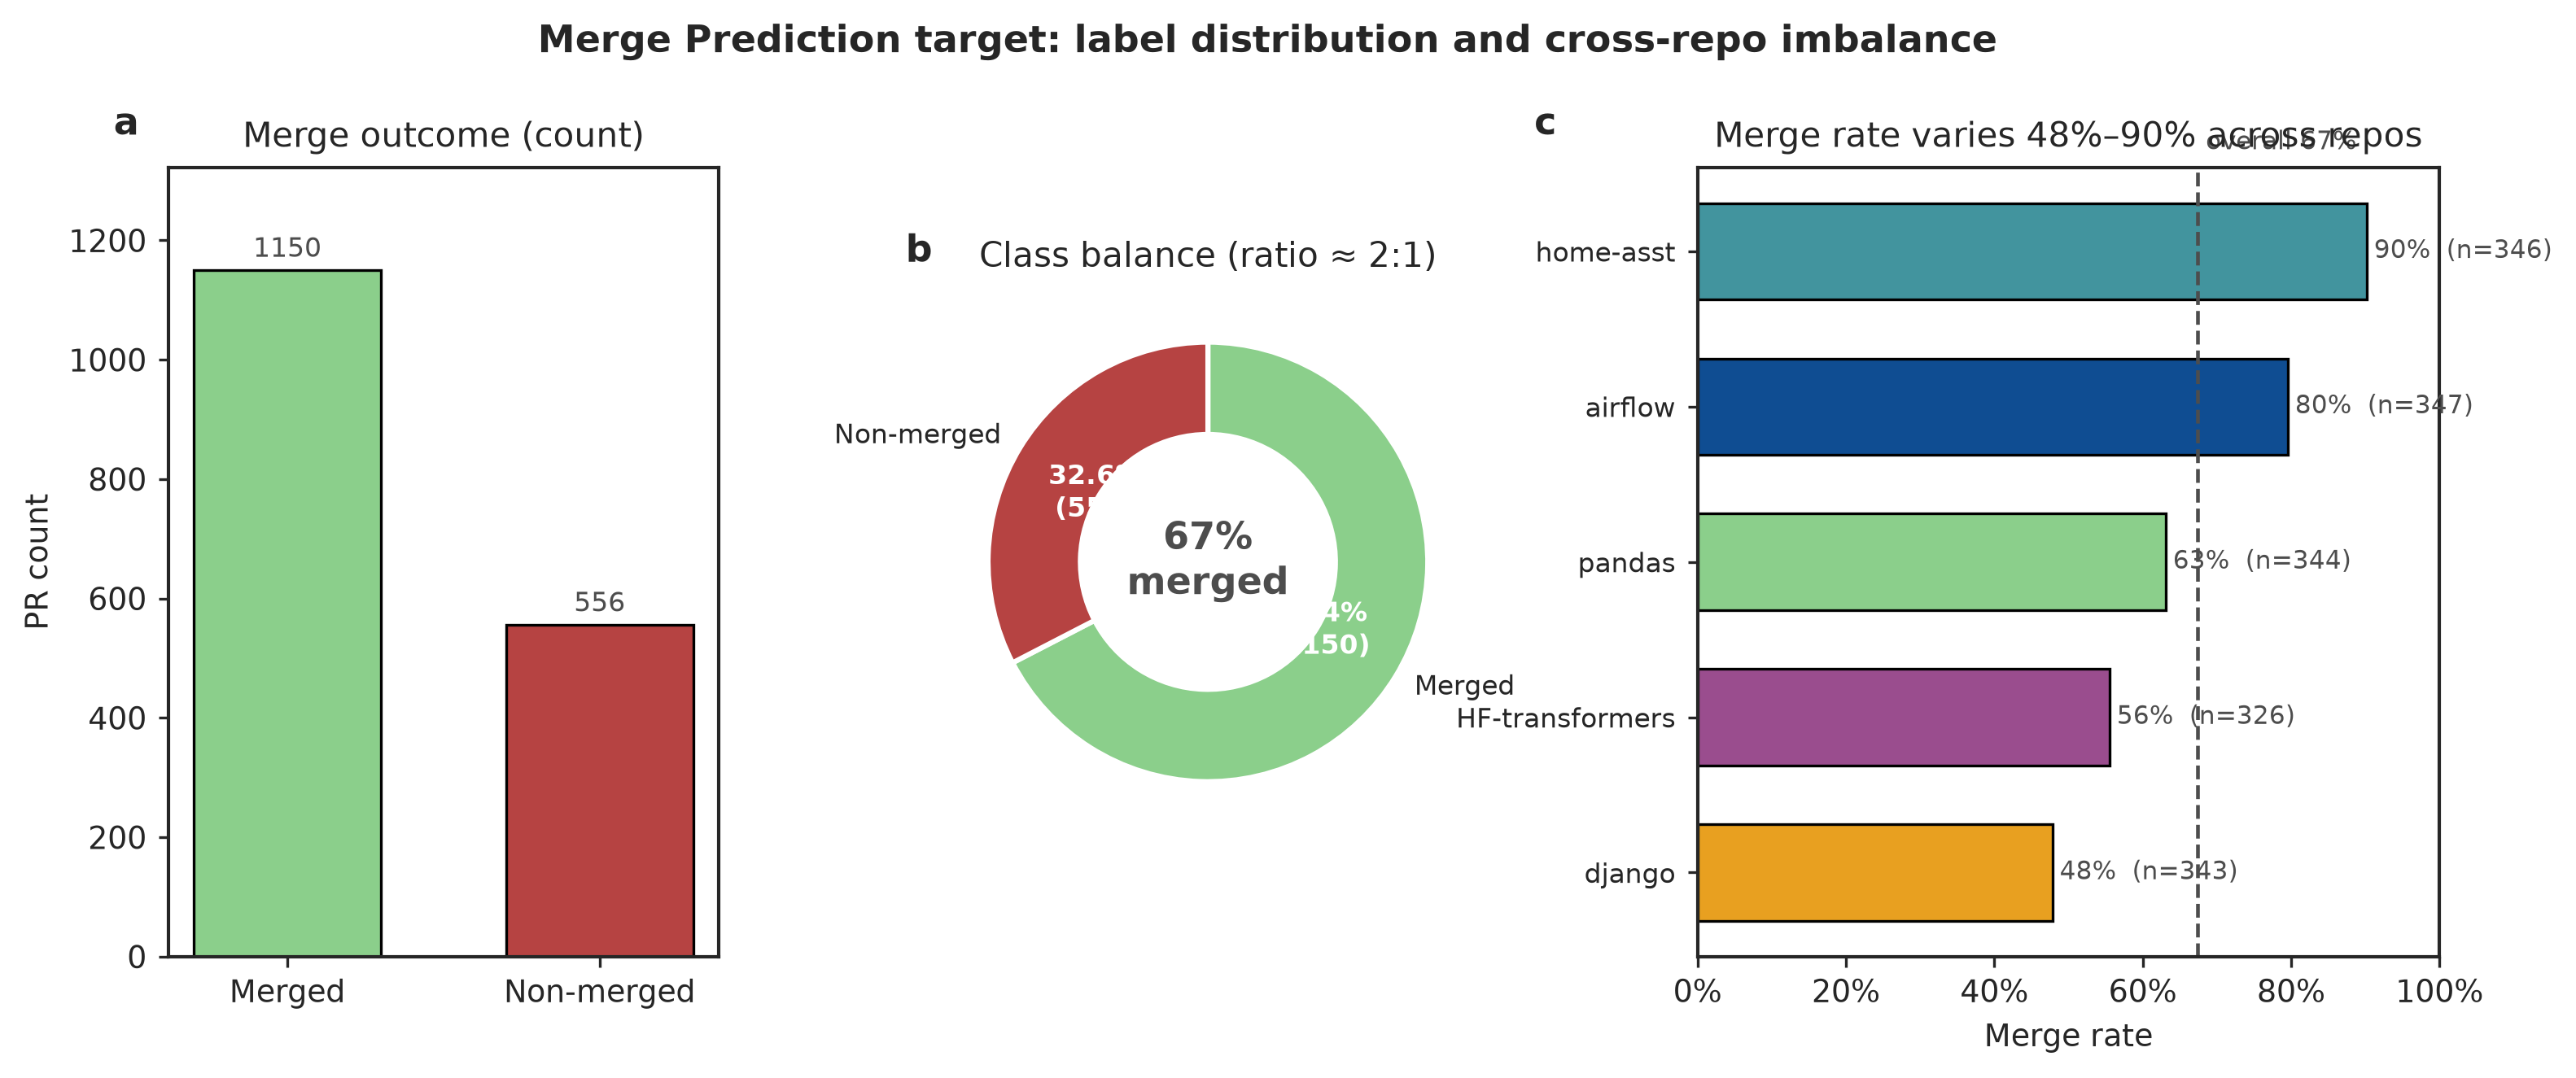
\includegraphics[width=\textwidth]{merge_vs_nonmerge.png}
\caption{\textbf{合并预测目标标签的分布与跨仓库差异。} (a) 合并与未合并 PR 数量（Merged $=1{,}150$，Non-merged $=556$）。(b) 类别占比，整体合并率 67.4\%，正负样本比约 2:1。(c) 各仓库合并率（升序排列），虚线为全局均值；合并率在 47.8\%（django）至 90.2\%（home-assistant）间变化，$n$ 标注于各条末端。}
\label{fig:merge}
\end{figure}

\subsection*{3.3 审查评论的稀疏性}

inline 审查评论是审查意见生成任务的唯一数据来源，其分布直接决定可用训练样本规模。绘制评论数直方图并按仓库统计"有评论 PR"占比（图~\ref{fig:comment}）。结果表明，评论分布呈现\textbf{极强的零膨胀}特征：73.9\% 的 PR 没有任何 inline 评论，中位数为 0，仅在尾部存在少量高评论 PR（p90 $=5$，p99 $=24$，最大 202 条）。社区层面，django 的审查密度最高（30.3\% 的 PR 含评论，均值 2.45 条）。

据此得出结论：仅约 26\% 的 PR（约 444 条）能够产生可用的 \texttt{(diff\_hunk $\rightarrow$ 审查意见)} 配对，这是生成任务实际可训练样本量的上界。因此实验三在准备数据时\textbf{必须先过滤} \texttt{num\_review\_comments $>0$}，否则将引入大量无标签噪声；若需高质量子集，可优先选取审查密度更高的 django 与 huggingface/transformers。

\begin{figure}[H]
\centering
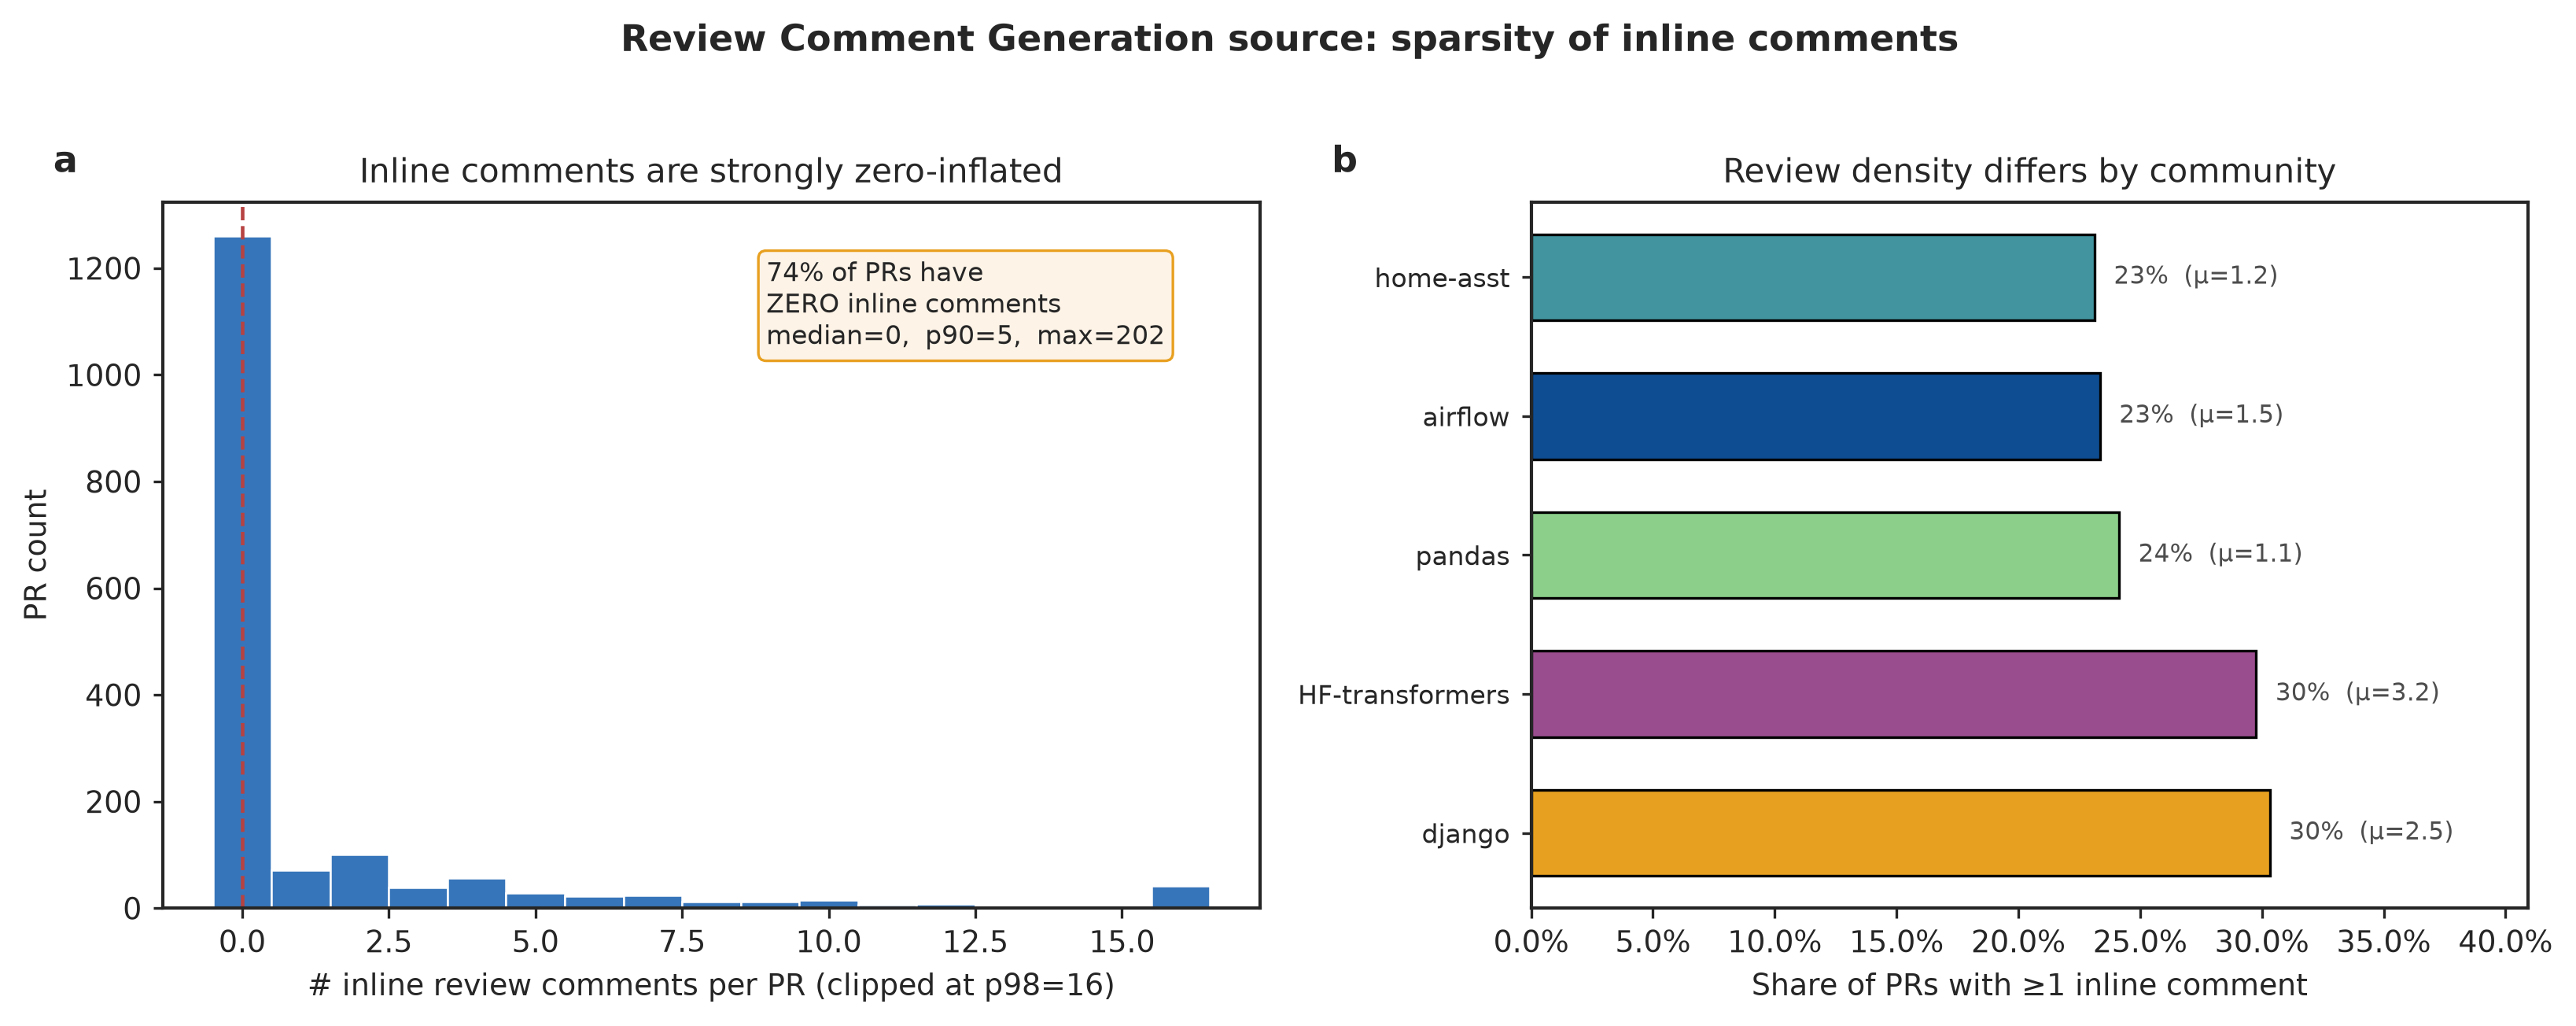
\includegraphics[width=\textwidth]{review_comment_dist.png}
\caption{\textbf{inline 审查评论的零膨胀分布与社区审查密度差异。} (a) 评论数直方图（截尾至 p98$=25$），73.9\% 的 PR 无任何 inline 评论。(b) 各仓库"有 $\geq 1$ 条 inline 评论"的 PR 占比，括号内 $\mu$ 为组内均值。}
\label{fig:comment}
\end{figure}

\subsection*{3.4 审查者数量与 PR 规模}

进一步考察审查投入与代码规模两个维度。审查者数量方面（图~\ref{fig:reviewer}），分布集中于 0--2 人（均值 1.30），且审查者数量与合并率呈显著正相关——无审查者的 PR 合并率仅 27.0\%，而拥有 2 名及以上审查者的 PR 合并率跃升至 92.6\%。这表明 \texttt{num\_reviewers} 是信息量很高的统计特征，实验二应优先纳入；但需注意其因果方向，审查者多是"PR 受重点关注"这一潜在变量的代理，而非合并的直接原因。

PR 规模方面（图~\ref{fig:size}），改动行数（additions + deletions）呈\textbf{典型重尾分布}，中位数仅 32 行，但 p90 达 339 行、p99 达 4{,}809 行、最大值近 97 万行，横跨约 6 个数量级，因此必须使用对数坐标。跨仓库看，pandas 因 PR 普遍附带大量测试与文档而规模最大。由此得出结论：所有规模类特征在建模前必须做对数变换（log1p）或分位数归一化，否则少数极端 PR 将主导 SVM 的距离度量与 CodeBERT 的 token 截断；对超过 p99 的巨型 PR 建议截断或单独标记。

\begin{figure}[H]
\centering
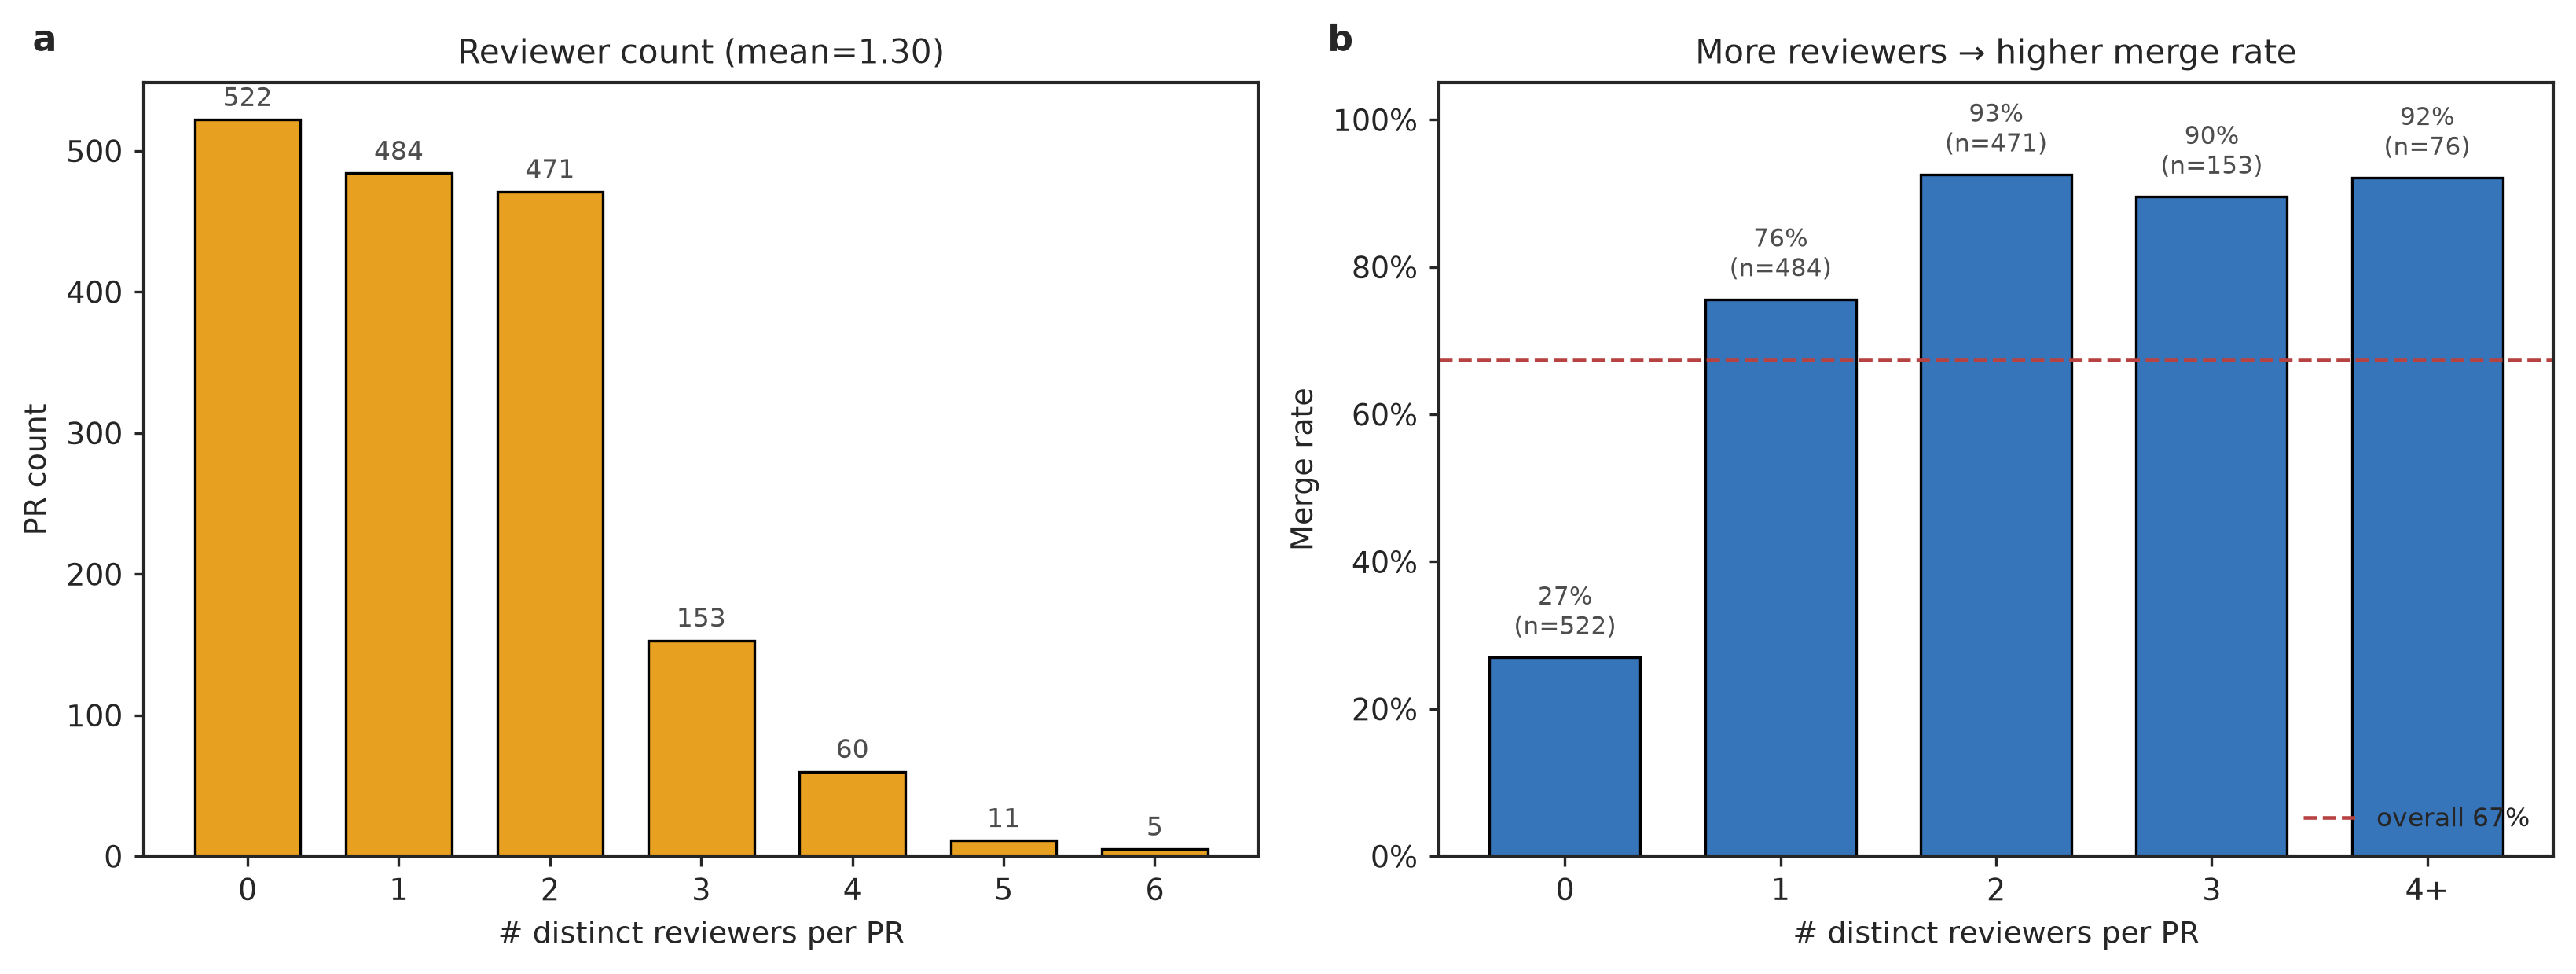
\includegraphics[width=\textwidth]{reviewer_dist.png}
\caption{\textbf{审查者数量分布及其与合并结果的关系。} (a) 每 PR 审查者数量分布（均值 $=1.30$）。(b) 按审查者数量分组的合并率，虚线为全局合并率；合并率随审查者数量从 27\% 升至 93\%。}
\label{fig:reviewer}
\end{figure}

\begin{figure}[H]
\centering
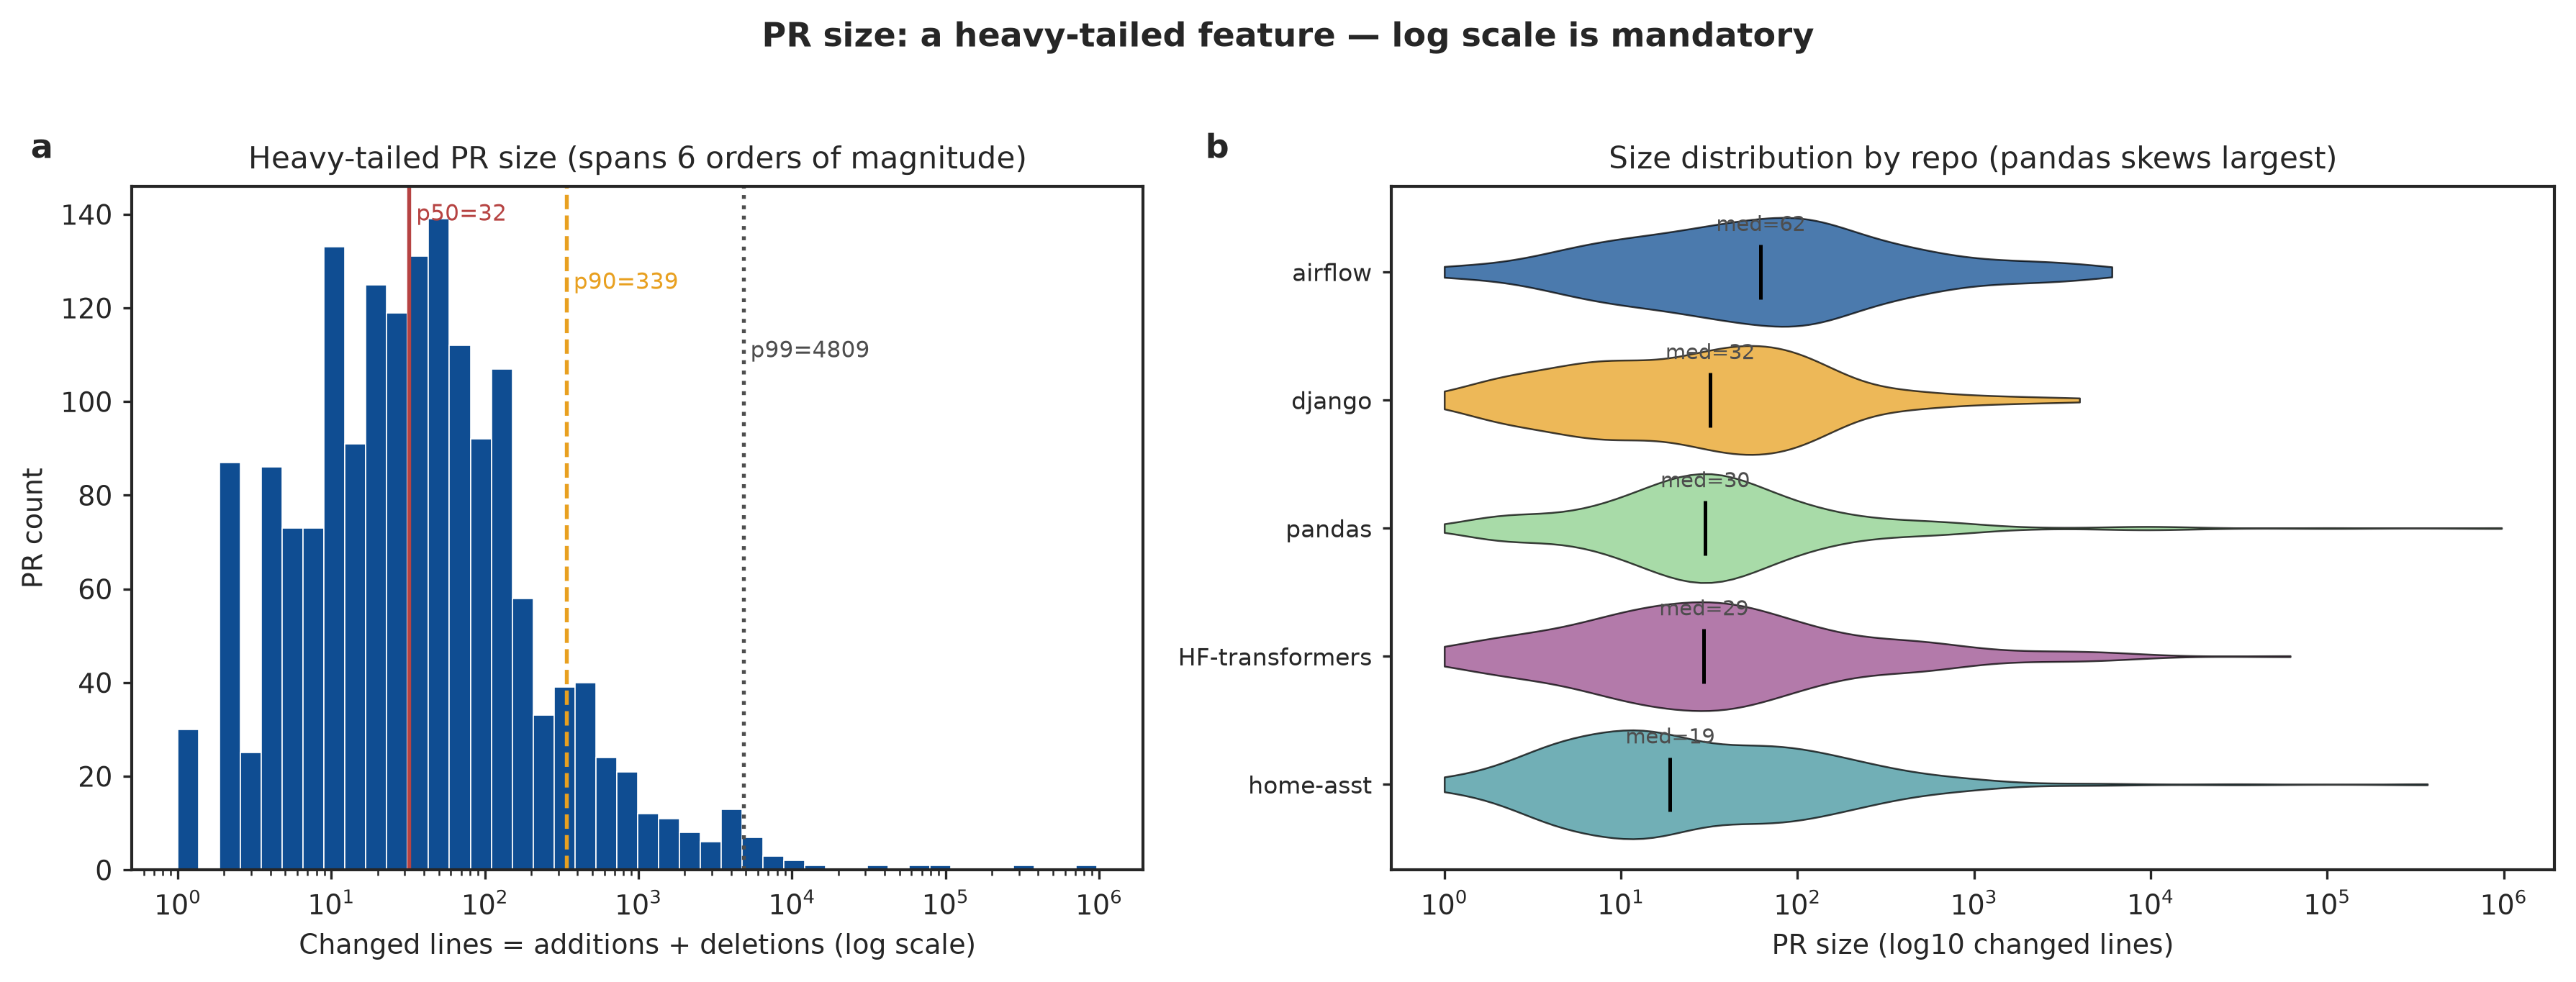
\includegraphics[width=\textwidth]{pr_size_dist.png}
\caption{\textbf{PR 改动规模的重尾分布及跨仓库差异。} (a) PR 规模对数直方图，竖线标注 p50$=32$、p90$=339$、p99$=4{,}809$ 行，分布横跨约 6 个数量级。(b) 各仓库 PR 规模小提琴图（$\log_{10}$ 尺度，按中位数升序），pandas 整体最大。}
\label{fig:size}
\end{figure}

\subsection*{3.5 AI 参与情况}

AI 标签是实验五的数据基础。统计 AI 代码信号构成，并对比 AI 与人类代码、有无 AI 审查者的合并率（图~\ref{fig:ai}）。结果显示：\texttt{is\_ai\_code} 的判定绝大多数来自强信号（commit 中的 \texttt{Co-authored-by} 达 376 次），标签整体可信度较高；最终 \texttt{is\_ai\_code=True} 达 294 条（17.2\%）、\texttt{has\_ai\_reviewer=True} 达 323 条（18.9\%），满足实验五需求。合并结果方面，AI 代码与人类代码合并率接近（71.8\% vs.\ 66.5\%），而有 AI 审查者的 PR 合并率（87.9\%）远高于无 AI 审查者者（62.6\%）。

需强调的是，AI 审查者与高合并率的强关联很可能是\textbf{选择效应而非因果}：323 条 AI 审查者样本中 301 条来自高合并率的 home-assistant 仓库。因此实验五在分析 AI 审查者效应时必须控制仓库这一混杂变量，不能直接归因于 AI 审查本身；同时，若需高精度 AI 代码子集，应通过 \texttt{ai\_code\_signals} 筛选强信号行。

\begin{figure}[H]
\centering
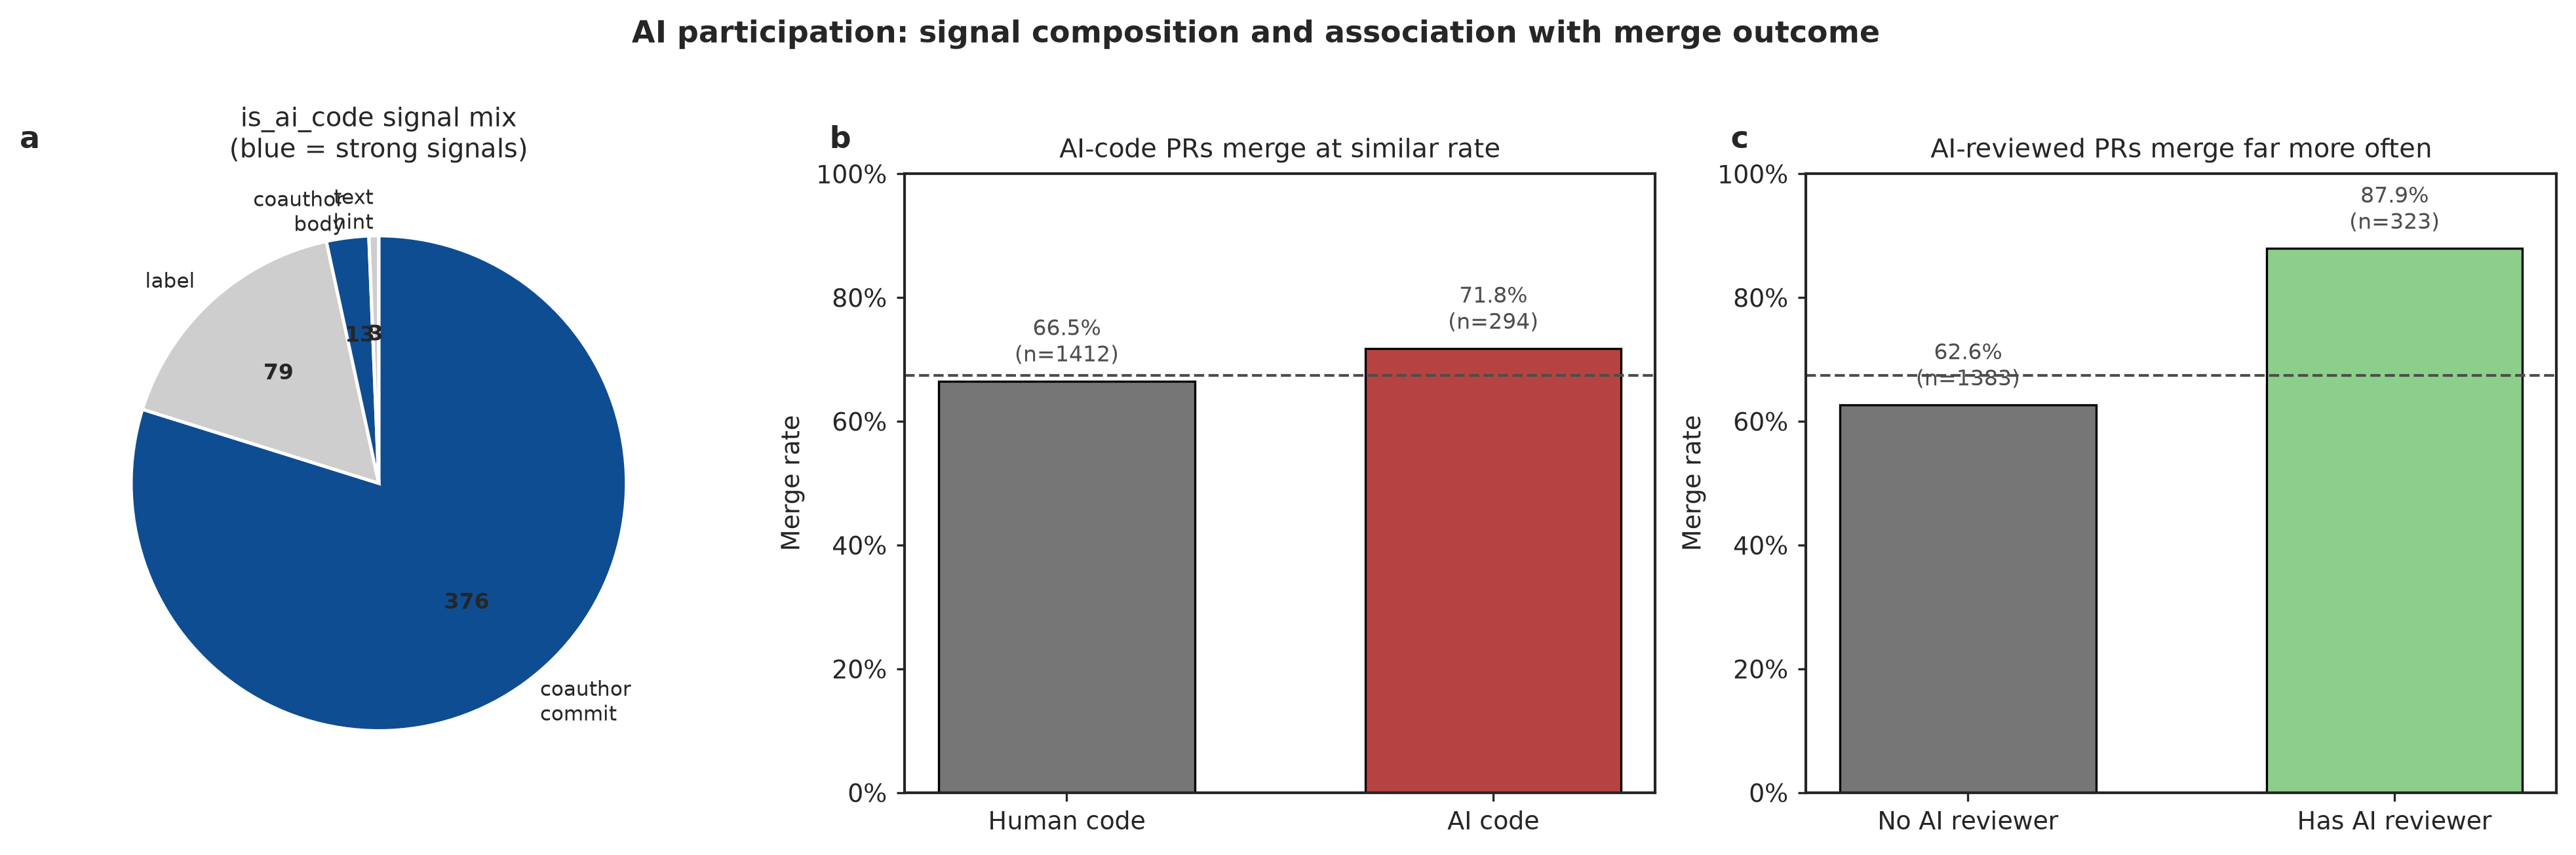
\includegraphics[width=\textwidth]{ai_vs_human.png}
\caption{\textbf{AI 参与度：信号构成及其与合并结果的关联。} (a) \texttt{is\_ai\_code} 命中信号类型构成（蓝色为强信号）。(b) AI 代码 vs 人类代码合并率。(c) 有无 AI 审查者的合并率对比；虚线为全局合并率。各柱标注合并率与样本量。}
\label{fig:ai}
\end{figure}

\subsection*{3.6 跨仓库对比}

最后从合并率、审查评论密度、PR 规模三个维度横向对比五个仓库（图~\ref{fig:cross}），以呼应实验一的拓展目标。三维度共同刻画出鲜明的社区画像：django 表现为"低合并率、高审查密度、小 PR"的高门槛精细审查文化；home-assistant 表现为"高合并率、低人工评论密度"的自动化审查文化；pandas 的 PR 规模最大；huggingface/transformers 则合并率偏低但评论密度最高，社区讨论活跃而严格。

这一系统性的社区差异证实：将五个仓库简单混合成单一训练集会掩盖社区间的分布差异。因此后续所有建模实验都应将"仓库"作为分层或协变量因素处理，并在评估时报告分仓库指标，而非仅看整体平均。综合 3.1--3.6 的分析可以确认，本数据集在规模、标签质量、分布多样性与时间跨度上均满足要求，可作为后续六个实验统一、可靠的数据基础。

\begin{figure}[H]
\centering
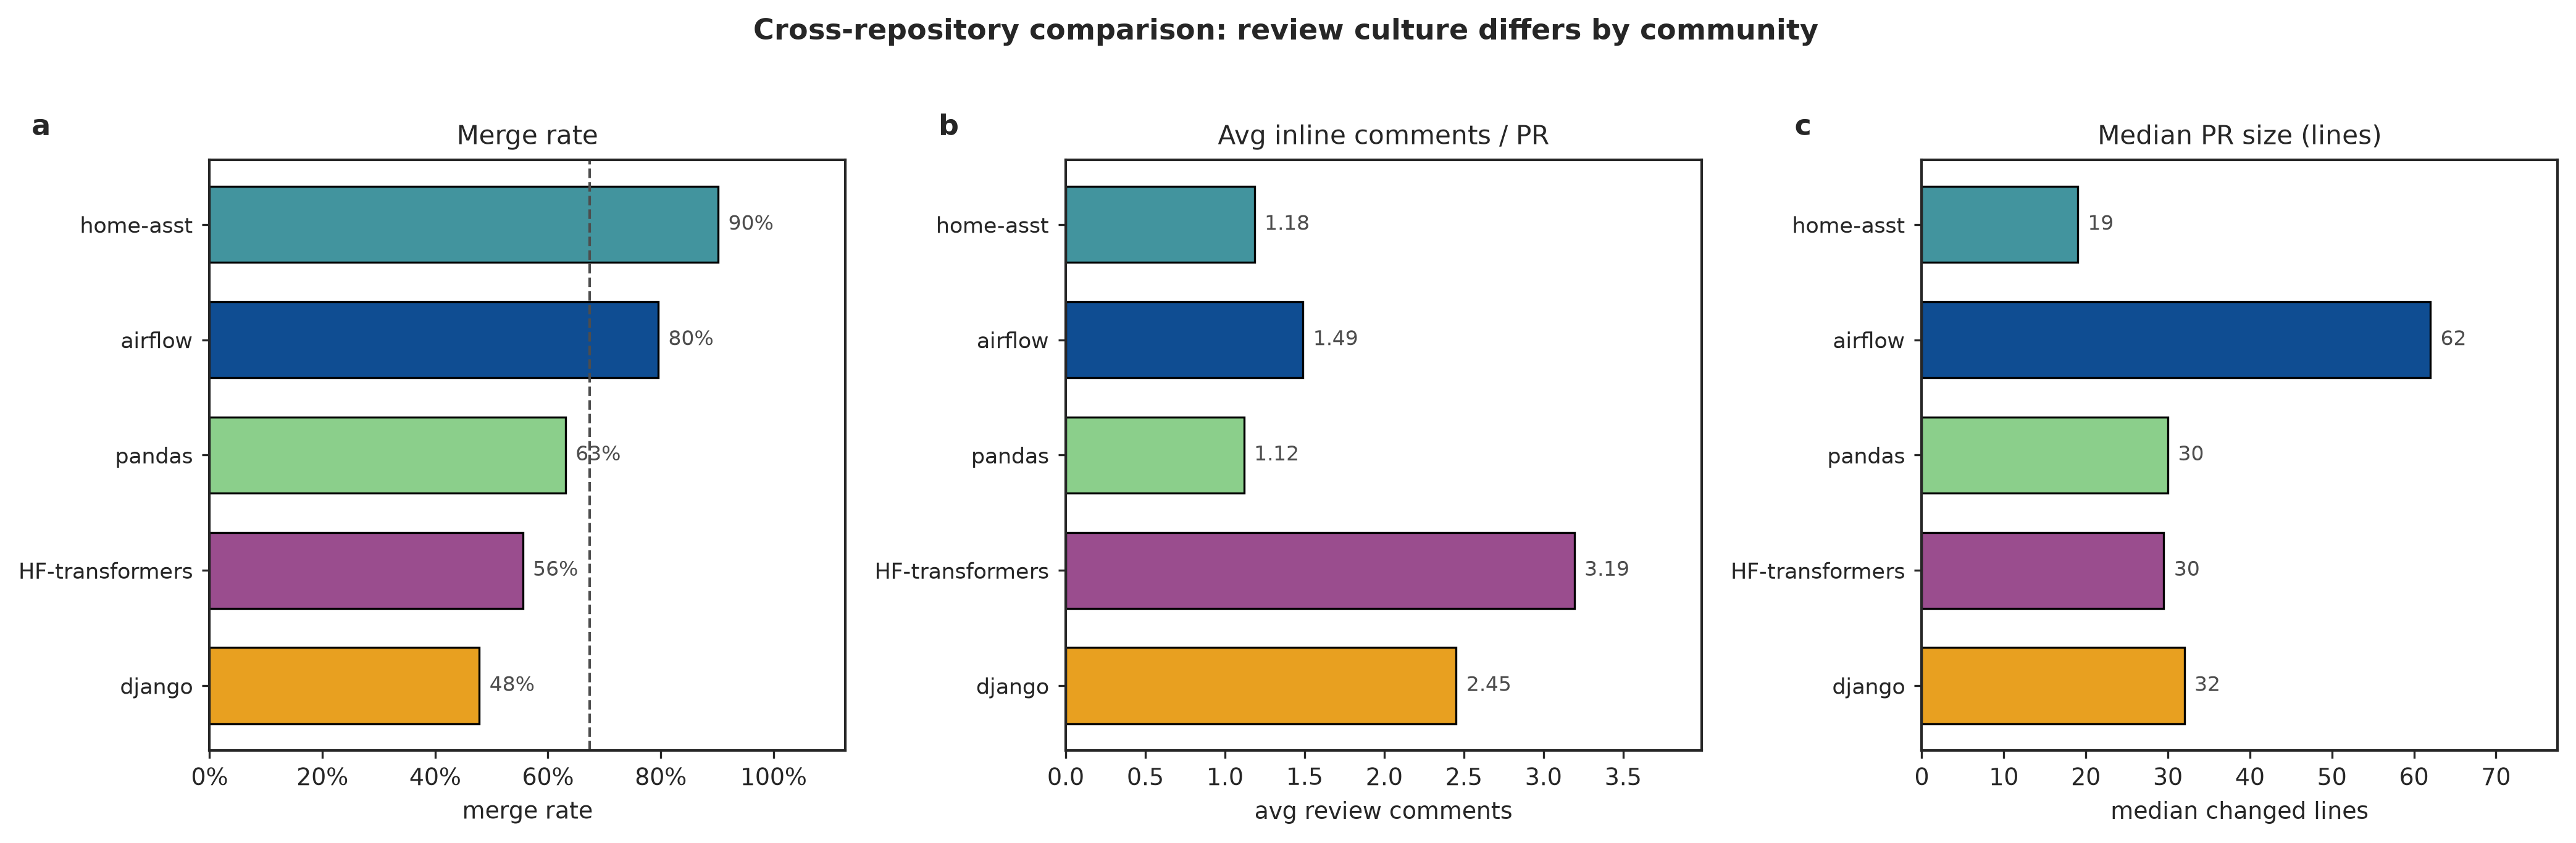
\includegraphics[width=\textwidth]{cross_repo.png}
\caption{\textbf{跨仓库多维对比：不同社区的代码审查文化差异。} 三联横向条形图（各仓库按合并率升序，配色跨图一致）：(a) 合并率，虚线为全局均值；(b) 每 PR 平均 inline 评论数；(c) PR 规模中位数。$N=1{,}706$，各仓库约 326--347 条。}
\label{fig:cross}
\end{figure}

}



%========================
% 问题总结
%========================

\experimentproblems{

\textbf{1. GitHub API 限流导致采集中断。}
采集初期未对 API 限额做主动监控，在连续抓取约 800 条 PR 后触发核心限额（5000 次/小时），程序阻塞报错退出。解决方案：在客户端封装中读取每次响应的 \texttt{X-RateLimit-Remaining} 与 \texttt{X-RateLimit-Reset} 头，额度低于阈值时精确休眠至重置时刻再继续；同时将每条 PR 独立存盘以支持断点续传，此后再无因限流导致的数据丢失。

\textbf{2. AI 生成代码样本极度稀少。}
五个仓库的基础 1{,}500 条随机样本中，自然出现的 \texttt{is\_ai\_code=True} PR 仅约 40 条，不足以支撑实验五的分析。解决方案：利用 GitHub Search API 定向搜索包含 AI 信号关键词的 PR（每仓库上限 50 条），在基础样本外补采 208 条，并以 \texttt{oversampled} 字段标记，最终将 AI 代码样本扩充至 294 条。

}

%========================
% 实验体会
%========================

\experimentexperience{

本实验最核心的收获是理解了"问题驱动的数据集设计"这一思路。在动手采集之前，花时间梳理后续六个实验对数据的隐含要求——生成任务需要带 \texttt{diff\_hunk} 的 inline 评论配对，AST/CFG 解析希望语言统一，实验五需要足量 AI 样本——这些前期约束直接决定了仓库选择标准、抓取粒度和表结构设计。

此外，探索性分析（EDA）的核心在于,在建模之前对数据风险的主动识别。合并率的 2:1 不平衡、评论分布的严重零膨胀、PR 规模的重尾特征，以及各仓库间超过 40 个百分点的合并率差距，这些在 EDA 阶段都已量化呈现；如果跳过这一步直接建模，这些问题将以更难排查的方式暴露在实验结果中；在数据获取后先进行一定的EDA并初步掌握数据原始特征是有一定价值的。

}

%========================
% 教师评语
%========================

\teachercomment

\end{document}
